\section{Implementation}
In implementation, you document the implementation (code) of the components from
design.
Describe the details of how the component are registered and accessed.
How are reliable dependencies and strong encapsulation enforced in your project?
What component models are applied and where in the source code?
Provide a descriptive explanation of each element in the implementation and 
provide arguments for your choices.
\\
\begin{figure}[H]
    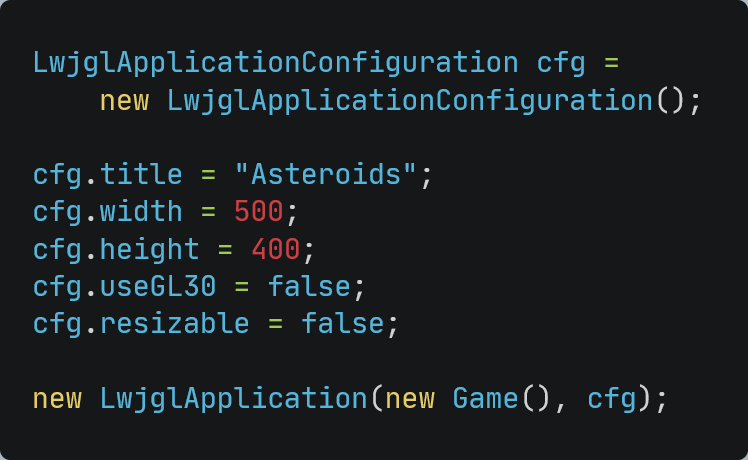
\includegraphics[width=\textwidth]{images/code/lwjgl2backend.png}
    \caption{Code from the Main.java file in the core module, as it looked when using the LWJGL2 backend.}
\end{figure}
\begin{figure}
    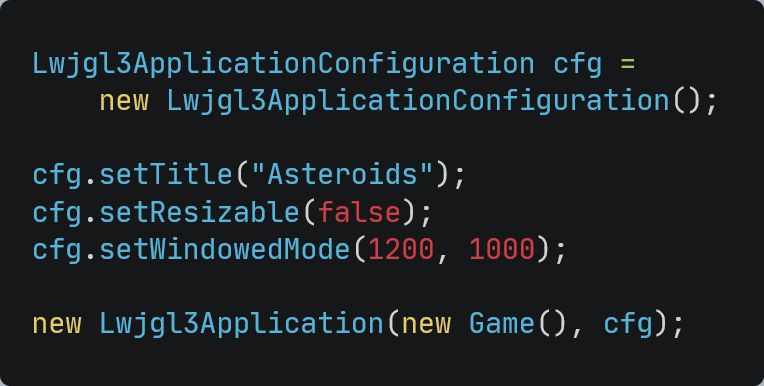
\includegraphics[width=\textwidth]{images/code/lwjgl3backend.png}
    \caption{Code from the Main.java file in the core module, as it looks when updated to the LWJGL3 backend.}
    
\end{figure}

Since the base example of the AsteroidsEntityFramework project made use of the
LWJGL2 backend as opposed to the LWJGL3 backend for handling rendering and audio
from LibGDX, an issue arose, where the example was possible. 